\documentclass{beamer}
\usepackage[english,russian]{babel}
\usepackage[utf8]{inputenc}
\usepackage{amsmath}
\usepackage{hyperref}
\usetheme{Warsaw}
\usepackage{listings}
\usepackage{xcolor}
\usepackage{tikz}
\usetikzlibrary{graphs}
\usepackage{algpseudocode}

\lstset{
    frame=tb,
    tabsize=4,
    showstringspaces=false,
    numbers=left,
    commentstyle=\color{green},
    keywordstyle=\color{blue},
    stringstyle=\color{red},
    emph={baz},
    emphstyle=\textbf
}

\begin{document}

\title{Задачи разрешимости логических формул и приложения\newline Лекция 7. Алгоритм Davis–Putnam–Logemann–Loveland(Theory).
Логики равенства и неинтерпритируемых функций}
\author{Роман Холин}
\institute{Московский государственный университет}
\date{Москва, 2021}

\begin{frame}
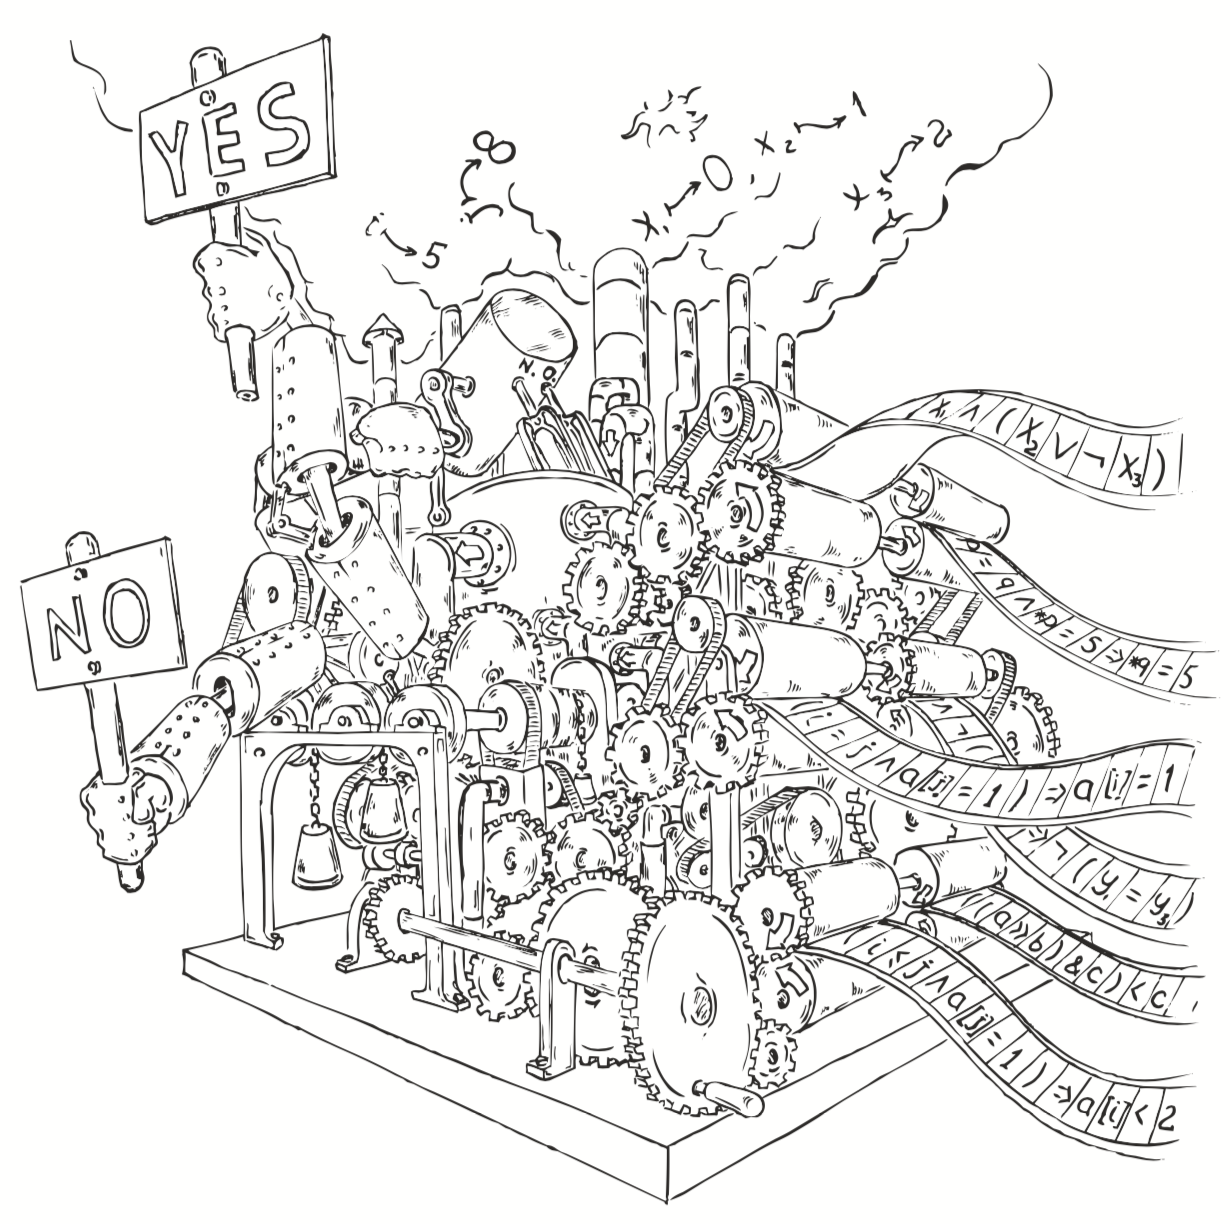
\includegraphics[scale=0.5]{../decision-procedure.png}
\end{frame}

\frame{\titlepage}

\begin{frame}{Ещё небольшая оптимизация CDCL}
\begin{itemize}
\item Во многих системах SAT решатель - лишь часть этой системы
\item Запросы к решателю могут быть похожи
\item Например, пусть есть робот, который нахоидтся на клеточном поле, которое является лабиринтом. Может ли робот выйти из него
за $k$ шагов?
\end{itemize}
\end{frame}

\begin{frame}{Ещё небольшая оптимизация CDCL}
\begin{itemize}
\item Во многих системах SAT решатель - лишь часть этой системы
\item Запросы к решателю могут быть похожи
\item Например, пусть есть робот, который нахоидтся на клеточном поле, которое является лабиринтом. Может ли робот выйти из него
за $k$ шагов?
\end{itemize}
Информацию можно использовать следующим образом:
\begin{itemize}
\item Использовать дизъюнкты
\end{itemize}
\end{frame}


\begin{frame}{Ещё небольшая оптимизация CDCL}
\begin{itemize}
\item Во многих системах SAT решатель - лишь часть этой системы
\item Запросы к решателю могут быть похожи
\item Например, пусть есть робот, который нахоидтся на клеточном поле, которое является лабиринтом. Может ли робот выйти из него
за $k$ шагов?
\end{itemize}
Информацию можно использовать следующим образом:
\begin{itemize}
\item Использовать дизъюнкты
\item Использовать эвристические параметры
\end{itemize}
\end{frame}

\begin{frame}{CDCL}
\begin{algorithmic}
\Function {CDCL}{}
    \While {true}
        \While {BCP() = "conflict"}
            \State backtrack-level := Analyze-Conflict()
            \If {backtrack-level < 0}
                \State return "Unsatisfiable"
            \EndIf
            \State BackTrack(backtrack-level)
            \If {$\lnot$ Decide()}
                \State return "Satisfiable"
            \EndIf
        \EndWhile
    \EndWhile
\EndFunction
\end{algorithmic}
\end{frame}

\begin{frame}{Lazy}
\begin{algorithmic}
\Function{Lazy}{$\phi$}
    \State $B := e(\phi)$
    \While {true}
        \State $<\alpha, res> := SAT-Solver(B)$
        \If {res = <<Unsatisfiable>>}
            \State return <<Unsatisfiable>>;
        \Else
            \State $<t, res> := Deduction(\overline{Th(\alpha)})$
            \If {res = <<Satisfiable>>}
                \State return <<Satisfiable>>
            \EndIf
            \State $B := B \wedge e(t)$;
        \EndIf
    \EndWhile
\EndFunction
\end{algorithmic}
\end{frame}

\begin{frame}

\includegraphics[scale=0.45]{pineapple}
\end{frame}

\begin{frame}
\begin{itemize}
\item Пусть $B_i$ - формула, которая получилась Lazy на $i$-ом шаге
\item По построению, $B_i$ - подформула $B_{i+1}$
\item Давайте не будем заново вызывать SAT решатель, а просто встроем в SAT решатель вызов решателя теории (и после вызова
решателя теорий будем добавлять блокирующий дизъюнкт)
\end{itemize}
\end{frame}

\begin{frame}{Lazy-CDCL}
\begin{algorithmic}
\State AddClauses(cnf(e($\phi$)))
\While {true}
    \While {BCP() = <<conflict>>}
        \State backtrack-level := Analyze-Conflict()
        \If {backtrack-level < 0}
            \State return <<Unsatisfiable>>
        \Else
            \State BackTrack(backtrack-level)
        \EndIf
        \If {$\lnot$ Decide()}
            \State $<t, res> := Deduction(\overline{Th(\alpha)})$
            \If {res = <<Satisfiable>>}
                \State return <<Satisfiable>>
            \EndIf
            \State AddClauses(e(t))
        \EndIf
    \EndWhile
\EndWhile
\end{algorithmic}
\end{frame}

\begin{frame}
\begin{itemize}
\item Что, если уже при данной частичной оценке формула в теории $T$ уже не выполнима?
\item Давайте всегда вызывать Deduction и добавлять к формуле невыолнимое ядро формулы
\end{itemize}
\end{frame}

\begin{frame}{Lazy-CDCL}
\begin{algorithmic}
\State AddClauses(cnf(e($\phi$)))
\While {true}
    \Repeat
        \While {BCP() = <<conflict>>}
            \State backtrack-level := Analyze-Conflict()
            \If {backtrack-level < 0}
                \State return <<Unsatisfiable>>
            \Else
                \State BackTrack(backtrack-level)
            \EndIf
            \State $<t, res> := Deduction(\overline{Th(\alpha)})$; AddClauses(e(t))
        \EndWhile
    \Until{t = true}
    \If {$\alpha$ is a full assignment}
        \State return <<Satisfiable>>
    \EndIf
    \State Decide()
\EndWhile
\end{algorithmic}
\end{frame}

\begin{frame}{Логика равенства}
$formula: formula \vee formula | \lnot formula | (formula) | atom$\newline
$atom: term = term$\newline
$term: identifier | constant$\newline
\end{frame}

\begin{frame}{Логика равенства (EQ)}
$formula: formula \vee formula | \lnot formula | (formula) | atom$\newline
$atom: term = term$\newline
$term: identifier | constant$\newline
Задача разрешимости формулы логики равенства - NP-полная\newline
\end{frame}

\begin{frame}{Удаление констант}
$\phi = \phi'$\newline
В $\phi'$ заменить все $c_i$ на $C_{c_i}$\newline
Для всех $i \neq j$ добавить в $\phi'$ формулы $C_{c_i} \neq C_{c_j}$
\end{frame}

\begin{frame}{Удаление констант}
$\phi' = \phi$\newline
В $\phi'$ заменить все $c_i$ на $C_{c_i}$\newline
Для всех $i \neq j$ добавить в $\phi'$ формулы $C_{c_i} \neq C_{c_j}$\newline
Далее будем считать, что в логике нет констант
\end{frame}

\begin{frame}{Логика неинтерпретируемых функций (UF)}
$formula: formula \vee formula | \lnot formula | (formula) | atom$\newline
$atom: term = term| predicateSymbol(list of terms)$\newline
$term: identifier | functionSymbol(list of terms)$\newline
\end{frame}

\begin{frame}{Логика неинтерпретируемых функций (UF)}
$formula: formula \vee formula | \lnot formula | (formula) | atom$\newline
$atom: term = term| predicateSymbol(list of terms)$\newline
$term: identifier | functionSymbol(list of terms)$\newline
Если predicateSymbol состоит только из \{=\}, то логику называют EUF
\end{frame}

\begin{frame}{Логика неинтерпретируемых функций(UF)}
Как используется?\newline
\end{frame}

\begin{frame}{Логика неинтерпретируемых функций(UF)}
Как используется?\newline
Если можем доказать в этой логике, то можем доказать и в общей фомруле
\end{frame}

\begin{frame}{Логика неинтерпретируемых функций(UF)}
Как используется?\newline
Если можем доказать в EUF, то можем доказать и в частной логике\newline
Обратное не верно: если формула не тавтология в EUF, то не факт, что это не тавтология в EUF
\end{frame}

\begin{frame}{Эквивалентность программ}
Программа a:\newline
int i, out\_a = in;\newline
for (int i = 0; i < 2; ++i) out\_a = out\_a * in;\newline
return out\_a;\newline
Программа b:\newline
int out\_b = (in * in) * in;\newline
return out\_b;\newline
\end{frame}

\begin{frame}{Эквивалентность программ}
Программа a:\newline
int i, out\_a = in;\newline
for (int i = 0; i < 2; ++i) out\_a = out\_a * in;\newline
return out\_a;\newline
Программа b:\newline
int out\_b = (in * in) * in;\newline
return out\_b;\newline
$\phi_a := (out\_a_0 = in\_a_0) \wedge (out\_a_1 = out\_a_0 * in\_a_0) \wedge (out\_a_2 = out\_a_1 * in\_a_0)$\newline
$\phi_b := out\_b_0 = (in\_b_0 * in\_b_0) * in\_b_0$\newline
Чтобы программы были эквивалентны, должно выполняться:\newline
$(in\_a_0 = in\_b_0) \wedge \phi_a \wedge \phi_b \rightarrow out\_a_2 = out\_b_0$
\end{frame}

\begin{frame}{Эквивалентность программ}
Программа a:\newline
int i, out\_a = in;\newline
for (int i = 0; i < 2; ++i) out\_a = out\_a * in;\newline
return out\_a;\newline
Программа b:\newline
int out\_b = (in * in) * in;\newline
return out\_b;\newline
Перепишем формулу в EUF. Будем считать, что * - это некоторый двуместный функциональный символ G(,)
\end{frame}

\begin{frame}{Эквивалентность программ}
Программа a:\newline
int i, out\_a = in;\newline
for (int i = 0; i < 2; ++i) out\_a = out\_a * in;\newline
return out\_a;\newline
Программа b:\newline
int out\_b = (in * in) * in;\newline
return out\_b;\newline
Перепишем формулу в EUF. Будем считать, что * - это некоторый двуместный функциональный символ G(,)
$\phi_a := (out\_a_0 = in\_a_0) \wedge (out\_a_1 = G(out\_a_0, in\_a_0)) \wedge (out\_a_2 = G(out\_a_1, in\_a_0)$\newline
$\phi_b := out\_b_0 = G(G(in\_b_0, in\_b_0), in\_b_0)$\newline
Чтобы программы были эквивалентны, должно выполняться:\newline
$(in\_a_0 = in\_b_0) \wedge \phi_a \wedge \phi_b \rightarrow out\_a_2 = out\_b_0$, но теперь нам не нужно знать природу G
\end{frame}

\begin{frame}{Замыкание классов эквивалентности}
\begin{itemize}
\item Построить замыкание классов эквивалентности:\newline
Поместить в один класс эквивалентности термы, если $t_1 = t_2$\newline
Слить все в один класс эквивалентности формулы $F(t_i)$, такие что $F(t_i) = F(t_j)$ и $t_i$ и $t_j$ в одном классе
эквивалентности\newline
Повторять, пока есть что сливать
\item Если какие-то $\phi_i$ и $\phi_j$ в одном классе эквивалентности и есть неравенство $\phi_i \neq \phi_j$, то вернуть результат
<<Unsatisfiable>>. Иначе вернуть <<Satisfiable>>
\end{itemize}
\end{frame}

\begin{frame}
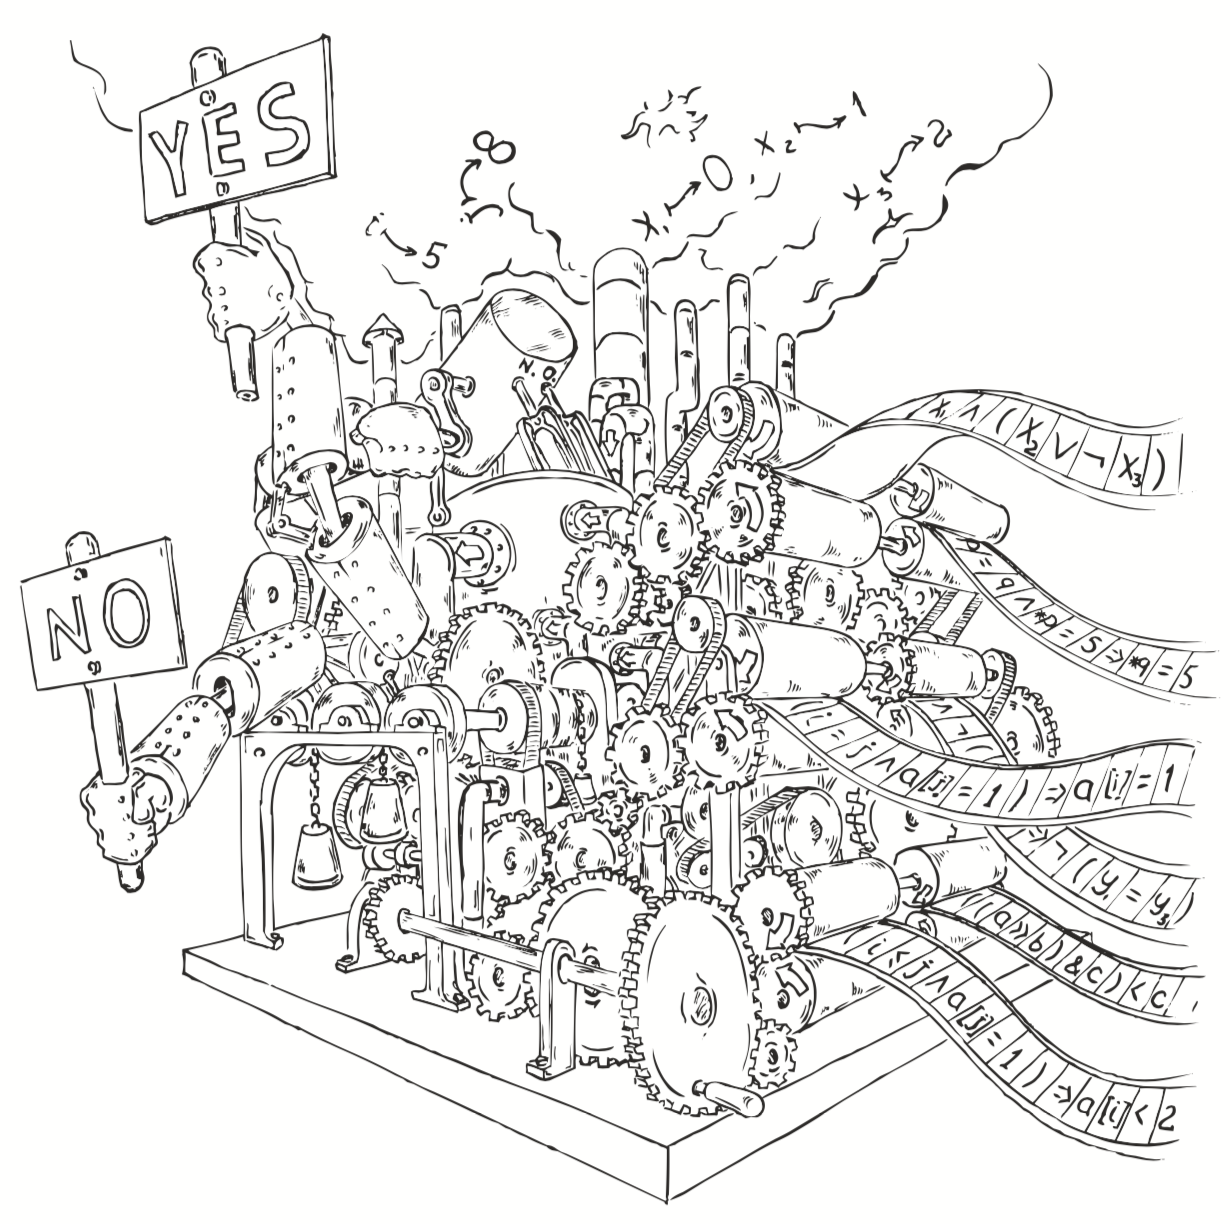
\includegraphics[scale=0.5]{../decision-procedure.png}
\end{frame}

\end{document}
